\documentclass[aspectratio=169]{beamer}
\usepackage[T1]{fontenc}
\usepackage[utf8]{inputenc}
\usepackage{lmodern}
\usepackage[french]{babel}
\usepackage{hyperref}
\usepackage{graphicx}
\usepackage{makecell}
\usepackage{xcolor}
\usepackage{colortbl}

\graphicspath{ {./img/} }

\newcommand{\TODO}{TODO:}
\newcommand*{\rot}{\rotatebox{90}}

\title{Bacula\\~\\AIT --- Présentation}
% \author{Cassandre Wojciechowski \\ Gwendoline Dössegger \\ Noémie Plancherel \\ Gaby Roch}
% \author{s}
\hypersetup{pdfauthor={C. Wojciechowski, G. Dössegger, N. Plancherel, G. Roch}}

\date{8 novembre 2021}

\begin{document}

\begin{frame}
  \titlepage
\end{frame}

\begin{frame}{Bacula -- Présentation général}
 \begin{itemize}
  \item Logiciel de sauvegarde multi-platform créé en 2000 par Kern Sibbald
  \item Première version 2002
  \item Dernière version 11.0.5, juin 2021
  \item Open source
 \end{itemize}
\end{frame}

\begin{frame}{Architecture}
 \begin{itemize}
  \item \TODO chiffré ??
  \begin{center}
  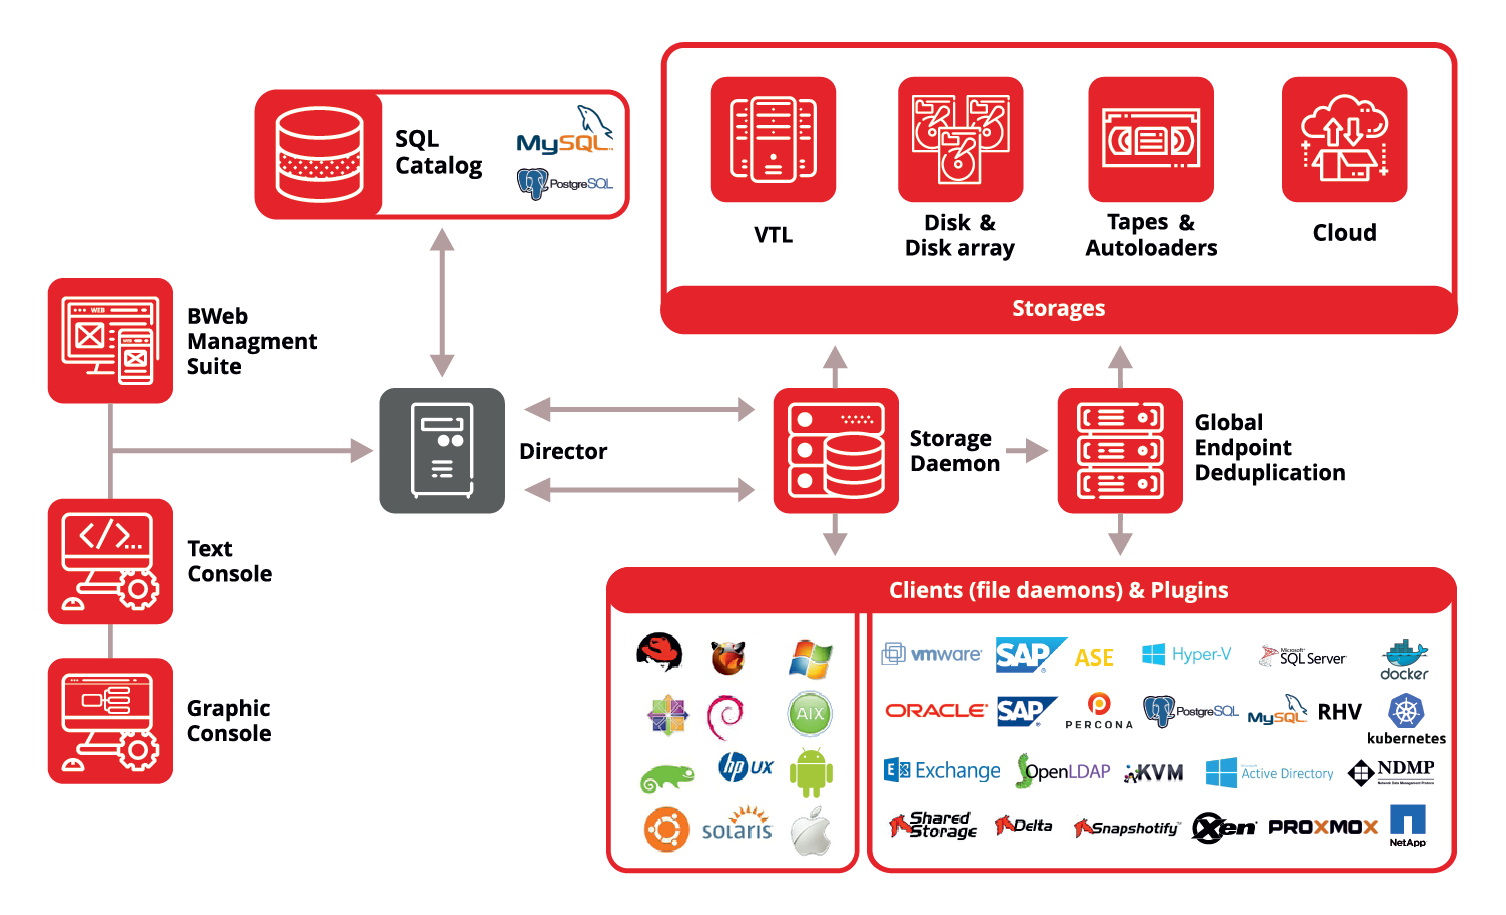
\includegraphics[height=60mm]{architecture.png}
   
  \end{center}

  
 \end{itemize}
\end{frame}

\begin{frame}{Demonstration}
 \begin{itemize}
  \item \TODO Temps de restauration de 1 fichier d'il y a 1 sem.
  \item 
 \end{itemize}
\end{frame}

\begin{frame}{Coût}
\begin{center}

 \begin{tabular}{|l|ccccc|}
    \hline
    & Standard & Bronze & Silver & Gold & Platinum \\
    \hline
    \hline
    Nombre de clients & < 50 & < 200 & < 500 & < 2000 & < 5000 \\
    \hline
    Nombre de contacts & 1 & 2 & 3 & 5 & 5 \\
    \hline
    Assistance & Web & Web & Web et tél.& Web et tél. & Web et tél. \\
    \hline
    Nombre d'OS & 4 & toutes & toutes & toutes & toutes \\
    \hline
    Temps de réponse & 1j -- 4j & 6h -- 4j & 4h -- 2j & 1h -- 2j & 1h -- 2j \\
    du support &  \\
    \hline
    Formation & 0 & 0 & 0 & 0 & 1/an \\
    \hline
 \end{tabular}
\end{center}

\TODO
2 version: - Community open source

Dès 500 \$ par mois sur devis pour la version Entreprise
\end{frame}


\begin{frame}{Comparaison}
 \begin{center}
  \begin{tabular}{|l||c|c|c|c|c|c|c|c|c|c|}
    \hline
    & Coût & \rot{Open source ~} & Backups & \rot{Déduplication ~} & \rot{Chiffrement ~} & \rot{Compression ~} & \rot{WI} & \rot{Linux} & \rot{MacOS X} & \rot{Windows} \\
    \hline
    \hline
    Bacula & \makecell{Gratuit\\payant} & \cellcolor{green!50} & \makecell{Full\\ incrémentaux\\ différentiels} & \cellcolor{green!50} & \cellcolor{green!50} & \cellcolor{green!50} & \cellcolor{green!50} & \cellcolor{black!50} & \cellcolor{black!50} & \cellcolor{black!50} \\
    \hline
    BorgBackup & \makecell{Gratuit\\payant} & \cellcolor{green!50} & \makecell{Full\\ incrémentaux\\ différentiels} & \cellcolor{green!50} & \cellcolor{green!50} & \cellcolor{green!50} & \cellcolor{orange!50} & \cellcolor{black!50} & \cellcolor{black!50} &  \\
    \hline
    Bup & Gratuit & \cellcolor{green!50} & Incrémentaux & \cellcolor{green!50} & \cellcolor{red!50} & \cellcolor{green!50} & \cellcolor{green!50} & \cellcolor{black!50} & \cellcolor{black!50} &  \\
    \hline
    Duplicati & Gratuit & \cellcolor{green!50} & \makecell{Full\\ incrémentaux} & \cellcolor{green!50} & \cellcolor{green!50} & \cellcolor{green!50} & \cellcolor{green!50} & \cellcolor{black!50} & \cellcolor{black!50} & \cellcolor{black!50} \\
    \hline
    Rsync & Gratuit & \cellcolor{green!50} & Incrémentaux & \cellcolor{red!50} & \cellcolor{red!50} & \cellcolor{red!50} & \cellcolor{red!50} & \cellcolor{black!50} & \cellcolor{black!50} & \cellcolor{black!50}  \\
    \hline
 \end{tabular}
 \end{center}
\end{frame}

\begin{frame}{Avantage / incovéniant}
 \TODO optimisation backup réseau + CPU
    \begin{center}
     \begin{tabular}{|l|l|}
     \hline
      \textbf{Avantages} & \textbf{Inconvénients} \\
     \hline
     \hline
        Cross-platform & Prise en main complexe \\
     \hline
      Automatisation \& scheduling & Pas de scan de virus\\
     \hline
     Toujours maintenu  & Courbe d'apprentissage plutôt raide \\
     (dernière update: juin 2021) & (configurations) \\
     \hline
     Détection d'erreurs & \\
     \hline
     Cloud \& backup hors site & \\
     \hline
     Deduplication efficiante & \\
     (accélere le backup) & \\
     \hline
     Support d'environment virtuel & \\
     \hline
     Documentation multi-langue & \\
     \hline
     \end{tabular}

    \end{center}

\end{frame}

\begin{frame}{Discussion stratégique}
 \begin{itemize}
  \item \TODO Quel médium de backup supporter ?
  \item \TODO RPO ?
  \item \TODO Backup full automatique
  \item \TODO Support des devices déconnecter
 \end{itemize}
\end{frame}

\begin{frame}{Question ?}
 \begin{itemize}
  \item 
 \end{itemize}
\end{frame}


\end{document}
